\documentclass{beamer}
\usetheme{Singapore}
\usepackage[round,sort]{natbib}
\usepackage{tikz}
\usetikzlibrary{arrows,decorations.pathmorphing,backgrounds,fit,positioning,shapes.symbols,chains}
\usepackage{adjustbox}
\usepackage{verbatim}
\usepackage{graphicx}
\graphicspath{ {etig-05-aiyenggar-images/} }

\title{Diffusion of Innovation}
\subtitle{A Review of Readings}
\author{Ashwin Iyenggar}
\institute[Indian Institute of Management Bangalore] 
{
  Corporate Strategy and Policy\\
  Indian Institute of Management Bangalore
}
\date{28 January, 2017}
\subject{Review of Assigned Readings on bridging the macro \& and micro aspects of innovation}

% \pgfdeclareimage[height=0.5cm]{university-logo}{university-logo-filename}
% \logo{\pgfuseimage{university-logo}}

\AtBeginSubsection[]
{
  \begin{frame}<beamer>{Outline}
    \tableofcontents[currentsection,currentsubsection]
  \end{frame}
}

\begin{document}

\begin{frame}
  \titlepage
\end{frame}

\begin{frame}{Outline}
  \tableofcontents
  % You might wish to add the option [pausesections]
\end{frame}

\section{Overview}
\begin{frame}{Bridging the micro and macro aspects of Innovation}{}
\begin{itemize}
\item{General Purpose Technologies and Innovation}
\item{Diffusion of Innovation}
\item{Trade and Innovation}
\end{itemize}
\end{frame}

\begin{frame}{Diffusion of Innovation}{}
\begin{itemize}
\item{\cite{Stoneman2010} - Technological diffusion from demand and supply side, at different levels of analysis}
\item{\cite{Atkin2015} - Empirical study on organizational impediments to adoption of technology}
\item{\cite{Bollinger2012} - Empirical study of peer effects in technology diffusion}
\end{itemize}
\end{frame}






\section{\cite{Stoneman2010}}
\begin{frame}{The Diffusion of New Technology}{Agenda}
\begin{itemize}
\item{Scope of Definition of Technology Diffusion}
\item{Demand and Supply Side}
\item{Diffusion at different levels of aggregation - worldwide, industry, household}
\end{itemize}
\end{frame}

\begin{frame}{The Diffusion of New Technology}{Agenda}
\begin{figure}[h]
\begin{centering}
  \includegraphics[width=\textwidth]{stoneman1}
  \caption{Source: \cite{Stoneman2010}}
   \label{fig:stoneman1}
\end{centering}
\end{figure}
\end{frame}


\begin{frame}{The Diffusion of New Technology}{Agenda}
\begin{figure}[h]
\begin{centering}
  \includegraphics[width=\textwidth]{stoneman2}
  \caption{Source: \cite{Stoneman2010}}
   \label{fig:stoneman2}
\end{centering}
\end{figure}
\end{frame}




\section{\cite{Atkin2015}}
\begin{frame}{Organizational Barriers to Technology Adoption}{Summary}
\begin{itemize}
\item{Scope of Definition of Technology Diffusion}
\item{Demand and Supply Side}
\item{Diffusion at different levels of aggregation - worldwide, industry, household}
\end{itemize}
\end{frame}

\begin{frame}{Organizational Barriers to Technology Adoption}{Summary}
\begin{figure}[h]
\begin{centering}
  \includegraphics[width=\textwidth]{atkin1}
  \caption{Source: \cite{Atkin2015}}
   \label{fig:atkin1}
\end{centering}
\end{figure}
\end{frame}

\begin{frame}{Organizational Barriers to Technology Adoption}{Summary}
\begin{figure}[h]
\begin{centering}
  \includegraphics[width=\textwidth]{atkin2}
  \caption{Source: \cite{Atkin2015}}
   \label{fig:atkin2}
\end{centering}
\end{figure}
\end{frame}

\begin{frame}{Organizational Barriers to Technology Adoption}{Summary}
\begin{figure}[h]
\begin{centering}
  \includegraphics[width=\textwidth]{atkin3}
  \caption{Source: \cite{Atkin2015}}
   \label{fig:atkin3}
\end{centering}
\end{figure}
\end{frame}

\begin{frame}{Organizational Barriers to Technology Adoption}{Summary}
\begin{figure}[h]
\begin{centering}
  \includegraphics[width=\textwidth]{atkin4}
  \caption{Source: \cite{Atkin2015}}
   \label{fig:atkin4}
\end{centering}
\end{figure}
\end{frame}

\begin{frame}{Organizational Barriers to Technology Adoption}{Summary}
\begin{figure}[h]
\begin{centering}
  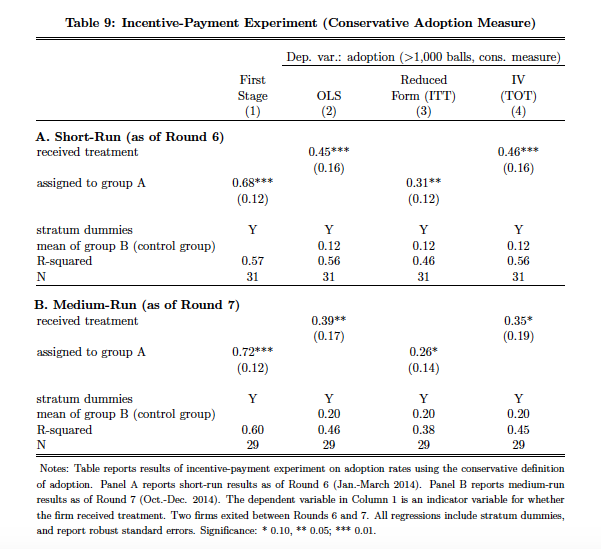
\includegraphics[width=\textwidth]{atkin5}
  \caption{Source: \cite{Atkin2015}}
   \label{fig:atkin5}
\end{centering}
\end{figure}
\end{frame}

\begin{frame}{Organizational Barriers to Technology Adoption}{Summary}
\begin{figure}[h]
\begin{centering}
  \includegraphics[width=\textwidth]{atkin6}
  \caption{Source: \cite{Atkin2015}}
   \label{fig:atkin6}
\end{centering}
\end{figure}
\end{frame}

\begin{frame}{Organizational Barriers to Technology Adoption}{Summary}
\begin{figure}[h]
\begin{centering}
  \includegraphics[width=\textwidth]{atkin7}
  \caption{Source: \cite{Atkin2015}}
   \label{fig:atkin7}
\end{centering}
\end{figure}
\end{frame}




\section{\cite{Bollinger2012}}
\begin{frame}{Peer Effects in Technology Diffusion}{Summary}
\begin{itemize}
\item{Proxy for property rights: Political Risk Services assessment of protection against government expropriation in a country, Polity IV's constraint on executive measure}
\end{itemize}
\end{frame}


\bibliography{/Users/aiyenggar/OneDrive/code/bibliography/ae,/Users/aiyenggar/OneDrive/code/bibliography/fj,/Users/aiyenggar/OneDrive/code/bibliography/ko,/Users/aiyenggar/OneDrive/code/bibliography/pt,/Users/aiyenggar/OneDrive/code/bibliography/uz}
\bibliographystyle{apalike}

\end{document}

\begin{comment}
\begin{figure}[h]
\begin{centering}
  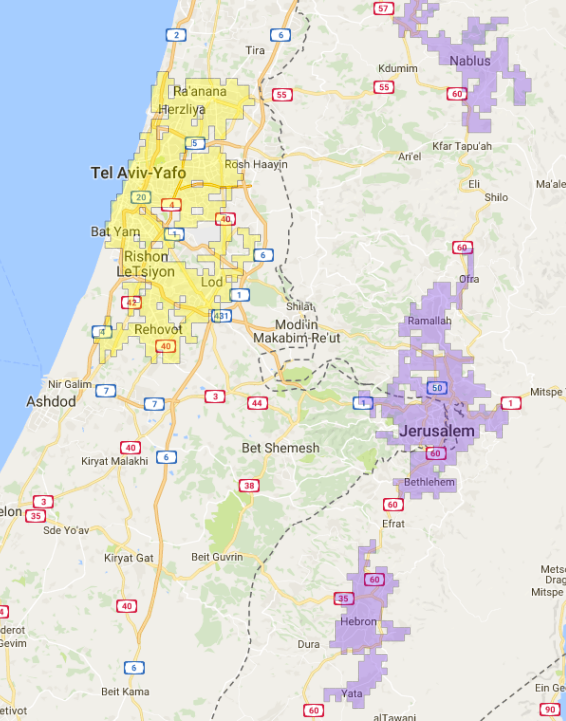
\includegraphics[width=\textwidth]{TelAviv}
  \caption{Geographic Definition of Tel Aviv-Yafo}
   \label{fig:TelAviv}
\end{centering}
\end{figure}
\end{comment}

